\chapter{Discusi\'on} 

Como explicamos al principio de este trabajo, existe evidencia de que es posible
parcelar el cerebro mediante un criterio funcional. Esto es, dividir el cerebro
en distintas regiones, atribuyendo una funci\'on a cada una de ellas \cite{Greicius2003}.
A su vez, la Resonancia Magn\'etica de Difusi\'on ha permitido desarrollar nuevos 
criterios estructurales de parcelaci\'on \cite{Taylor1985}. A lo largo de este
trabajo nos enfocamos en estudiar el reciente aporte de Moreno-Dominguez 
\cite{Moreno-Dominguez2014}. El mismo se basa en utilizar un algoritmo de
tractograf\'ia y otro de \textit{clustering} para parcelar la corteza cerebral. 
Luego, basandonos en su trabajo, propusimos un nuevo algoritmo de \textit{clustering},
tambi\'en basado en tractograf\'ias. En este \'ultimo capitulo discutiremos los 
resultados obtenidos. Comenzando por la robustes del algoritmo de tractograf\'ia
utilizado; siguiendo con una comparaci\'on entre nuestro m\'etodo y el de 
Moreno-Dominguez; luego hablaremos sobre la validez biol\'ogica de la parcelaci\'on
obtenida y propondremos objetos de futuro estudio. \\


\section{Convergencia del algoritmo de tractograf\'ia}

El algoritmo utilizado en el trabajo demostr\'o ser estable. Las figuras 
\ref{fig:s1}, \ref{fig:s2} y \ref{fig:s3} muestran que la desviaci\'on estandar
es casi nula al usar quince mil part\'iculas. A su vez, la figura \ref{fig:mv}
muestra lo r\'apido que converge la media de tres voxels distintos. Como eran los 
de mayor desv\'io estandar, podemos asegurar que casi no existe diferencia en 
la media de los tractogramas creados con dos mil part\'iculas. Nuestro m\'etodo
se basa en tractogramas, por lo que es importante contar con un algoritmo de 
tractograf\'ia robusto.

\section{Comparaci\'on entra ambos m\'etodos}

En ambos casos sucedi\'o que a mayor n\'umero $k$, menos dispersas quedaron las
distintas parcelas. Recordemos que $k$ es la cantidad de uniones que se har\'an
solo entre clusters vecinos. Respecto a las \'areas obtenidas, en la divisi\'on
del \'area de Broca los resultados fueron similares. La secci\'on \ref{sec:acercamiento} 
permite ver esto de manera explicita. Sin embargo, al pasar a la parcelaci\'on 
del hemisferio completo resulta dif\'icil realizar una simple comparaci\'on visual.
M\'as a\'un, es complicado encontrar cortes en los dendrogramas que generen 
representaciones parecidas. Sin embargo, en la secci\'on \ref{sec:acercamiento_corteza}
se puede ver que ambos resultados comparten similitudes. Por ejemplo, las 
siguientes estructuras son parecidas: la corteza motora y la somest\'esica; 
el lobulo frontal y occipital, as\'i como tambi\'en el \'area de Broca.


\section{Validaci\'on anat\'omica y funcional}

Dada la dificultad de comparar nuestro m\'etodo visualmente con el de Moreno-Dominguez
buscamos otra forma de validarlo. En la figura \ref{fig:an2pa} se puede ver
el resultado de proyectar la parcelaci\'on anat\'omica del sujeto sobre la que
obtuvimos. En interesante notar como nuestra parcelaci\'on cre\'o \'areas dentro
de los l\'imites de al menos 9 regiones an\'atomicas. En particular, la divisi\'on
del \'area motora parece ser consistente con la literatura actual. Por ello 
tambi\'en comparamos la parcelaci\'on con un estudio funcional hecho sobre el 
sujeto \cite{Barch2013}. 

\begin{figure}[h!]
    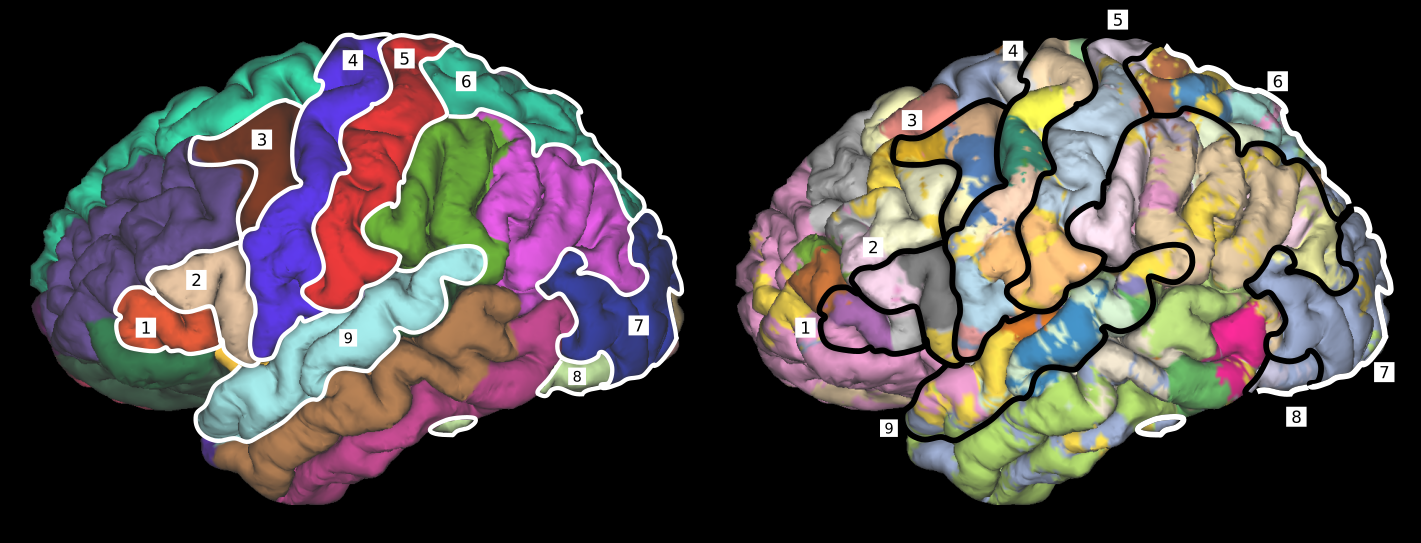
\includegraphics[width=\textwidth]{img/anatomica2parcelation.png}
    \caption{Proyecci\'on del atlas anat\'omico (izquierda) a la parcelaci\'on obtenida (derecha)}
    \label{fig:an2pa}
\end{figure}

\begin{figure}[h!]
    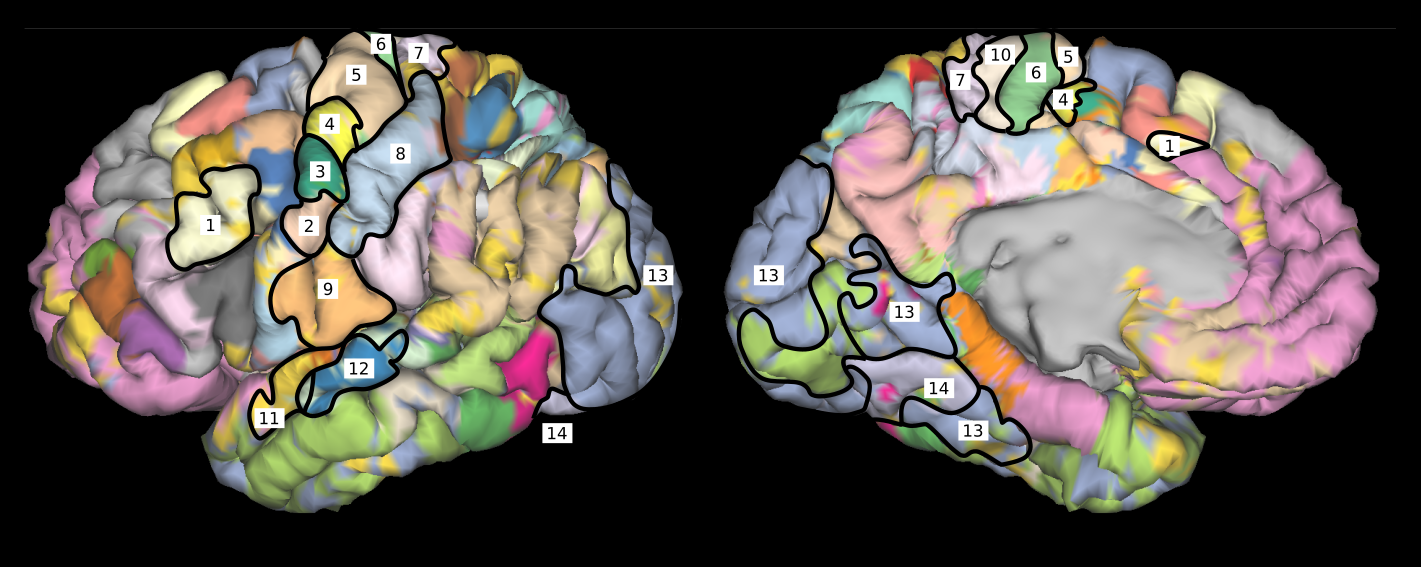
\includegraphics[width=\textwidth]{img/32k_labels.png}
    \caption{Parcelas en baja resoluci\'on}
    \label{fig:32k}
\end{figure}


\begin{figure}[h!]
    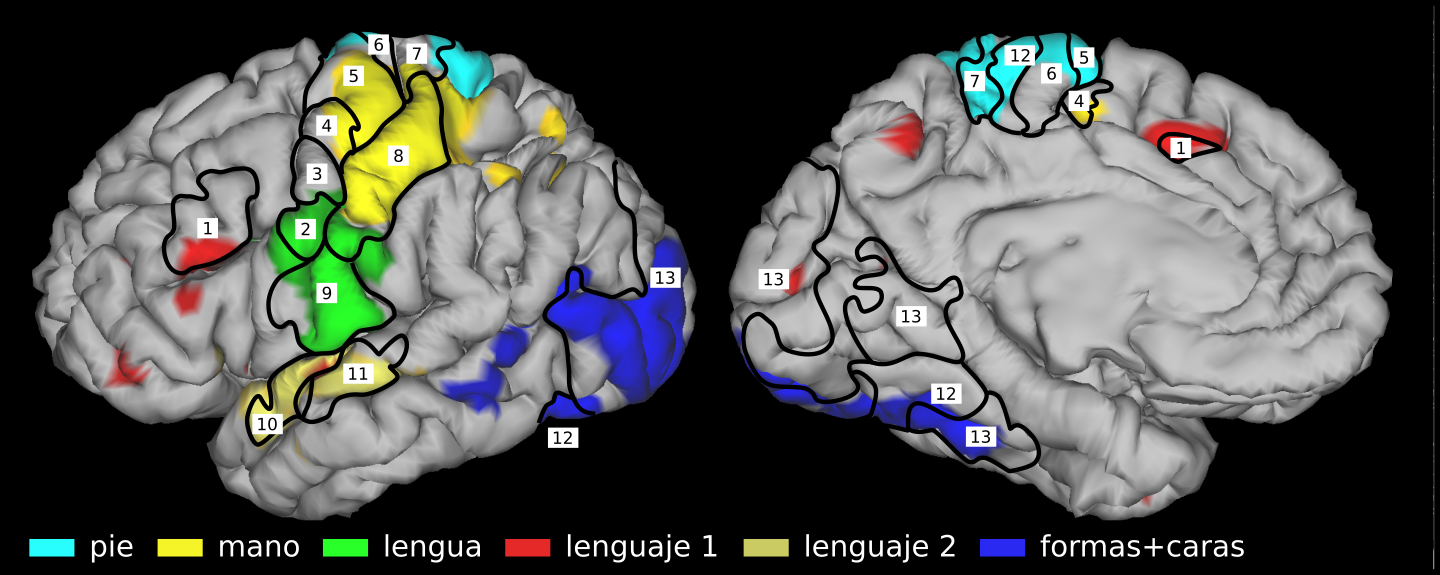
\includegraphics[width=\textwidth]{img/32k_z5.png}
    \caption{Projecci\'on de las parcelas (izquierda) sobre activaciones funcionales (derecha)}
    \label{fig:32k}
\end{figure}

\begin{figure}[h!]
    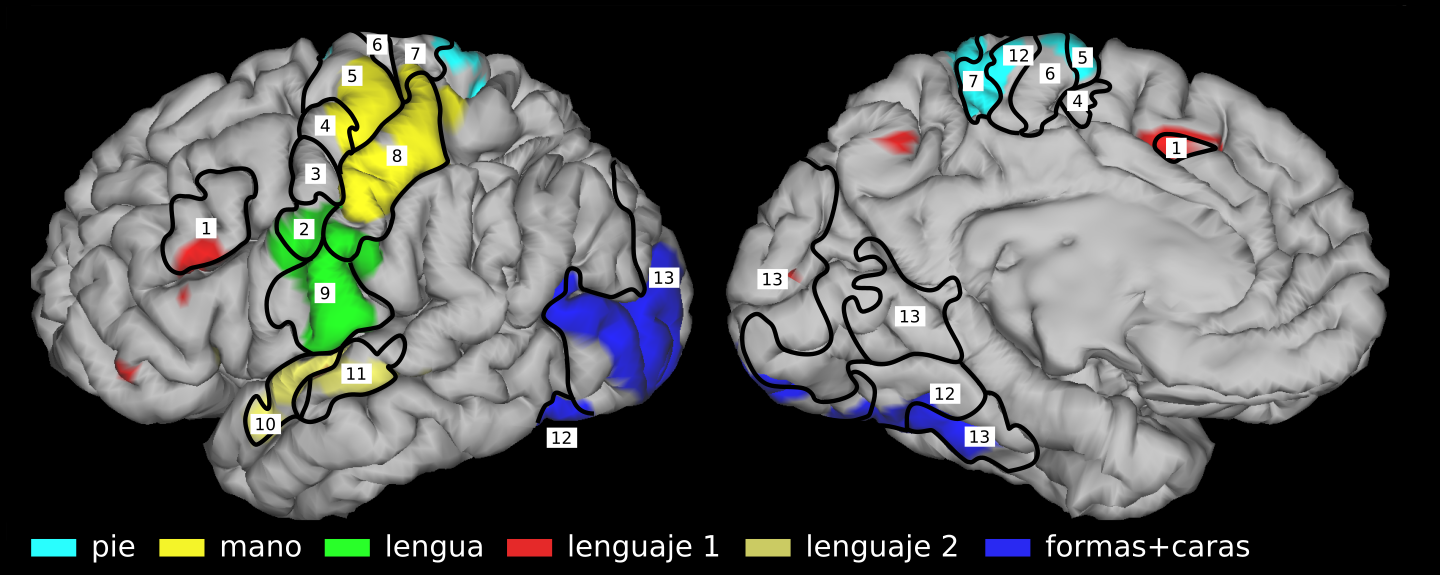
\includegraphics[width=\textwidth]{img/32k_z7.png}
    \caption{Projecci\'on de las parcelas (izquierda) sobre activaciones funcionales con 
             mayor valor de z-score (derecha)}
    \label{fig:32k}
\end{figure}
